\documentclass[12pt,a4paper]{article}

\usepackage[utf8]{inputenc}
\usepackage[spanish]{babel}
\usepackage[left=2.5cm,right=2.5cm,top=2.5cm,bottom=2.5cm]{geometry}

\usepackage[colorlinks = true, linkcolor = blue]{hyperref}
\usepackage{graphicx}
\usepackage{subfig}
\usepackage{listings}
\usepackage{url}

\author{Pablo Rodríguez Guillén \\ Profesor: Enrique García Salcines}
\title{\textbf{Fichero Aclaratorio Práctica 4: Expresiones regulares en Bash}}
\date{26 de mayo de 2019}

\setlength \parindent{0em}
\setlength \parskip{1em}

\begin{document}

\maketitle
\tableofcontents
\newpage

\section{ejercicio1.sh}
El ejercicio hace uso principalmente del comando \emph{grep} con algunas de sus opciones, principalmente la opción \emph{--colour} que hace que el patrón que coincida con la expresión regular se resalte con color en la salida de pantalla. El comando \emph{sed} también es utilizado en el último apartado del ejercicio. A la salida de este se le aplica un grep para resaltar las modificaciones.

Cada uno de los apartados está codificado en el fichero \emph{ejercicio1.sh} y la explicación concreta de cada uno está disponible a través de comentarios de \emph{bash}. Al inicio del script se encuentra la comprobación de errores al pasar el argumento, que debe ser un fichero. A continuación se muestra la primera parte de la ejecución del script, no se mostrará entera ya que la salida es extensa.

\begin{figure}[ht]
	\centering
	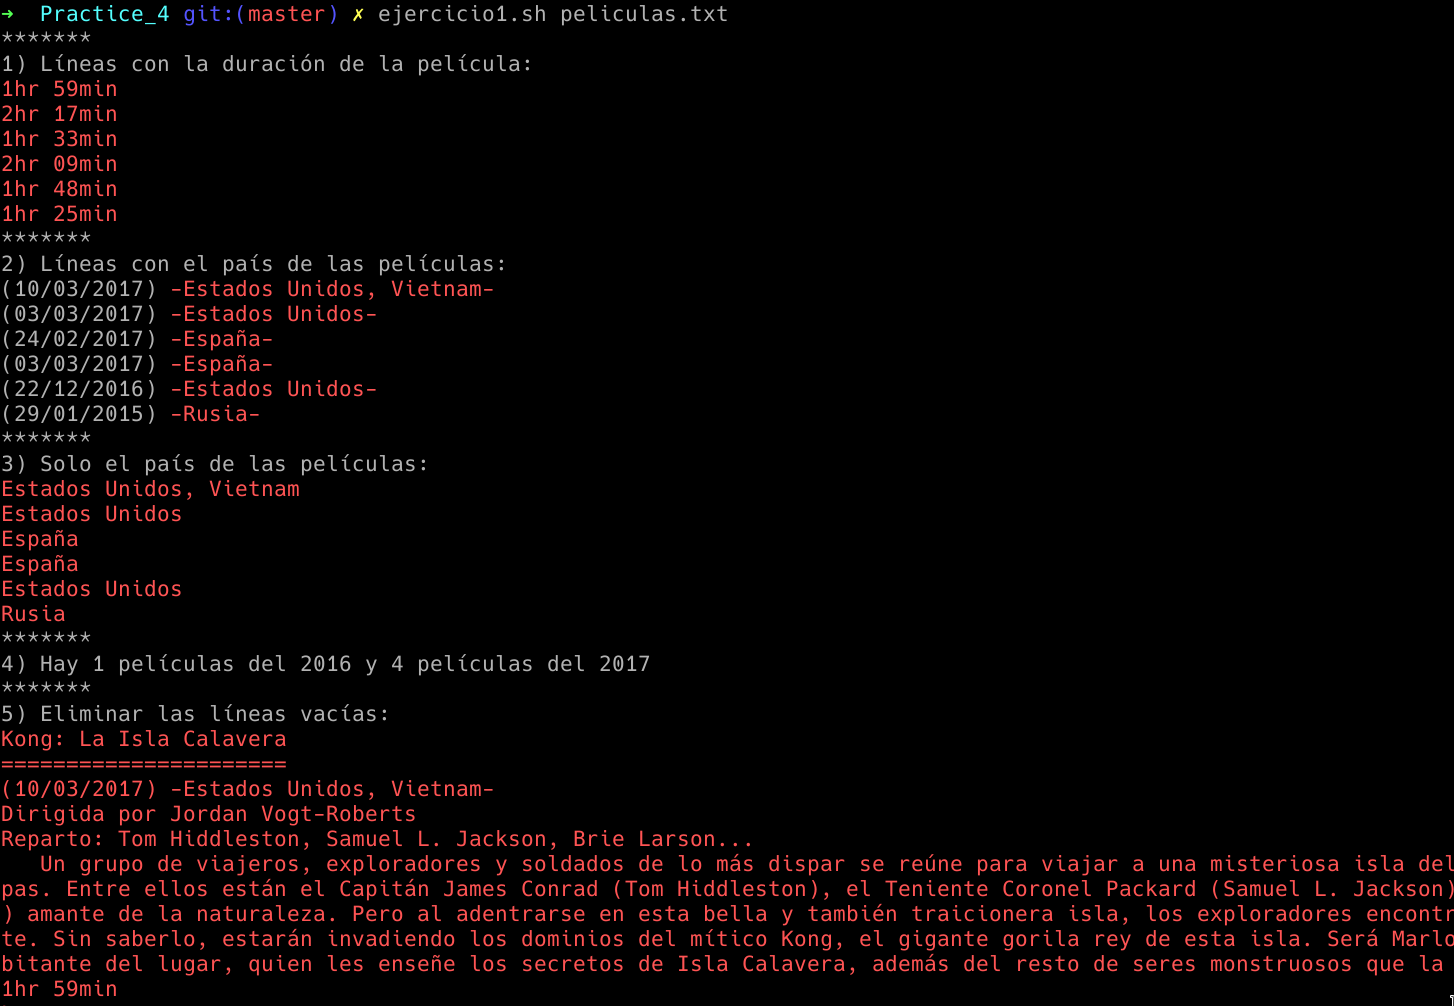
\includegraphics[width=1\textwidth]{images/ejercicio1.png}
	\caption{Salida de los 4 primeros apartados del ejercicio 1}
\end{figure}

\newpage

\section{ejercicio2.sh}
Este ejercicio comprueba que se le pasa un solo argumento por línea de comandos y que ese argumento, es la ruta de un fichero regular que existe en la máquina en la que se está ejecutando el script.

En primer lugar se hace un \emph{grep -v -E} que hace que se impriman las líneas que no coinciden con la expresión regular especificada. A esta salida se le aplica un \emph{sed} con varios comandos. El primero de ellos es un \emph{d}, que elimina las líneas que emparejan con la expresión regular precendente. El resto son comandos \emph{s} que tiene dos partes separadas por el carácter \emph{/}. La primera de ellas es una expresión regular en la que podemos crear una referencia para repetir el contenido de esta en la segunda parte. En esta segunda parte, especificamos la cadena que va a sustituir al texto que empareje con la expresión regular de la primera parte, recalcar que sustituye a la expresión entera no a la referencia. Esta referencia también puede llamarse argumento t se utiliza para repetir una parte de la cadena en la sustitución.

\begin{figure}[ht]
	\centering
	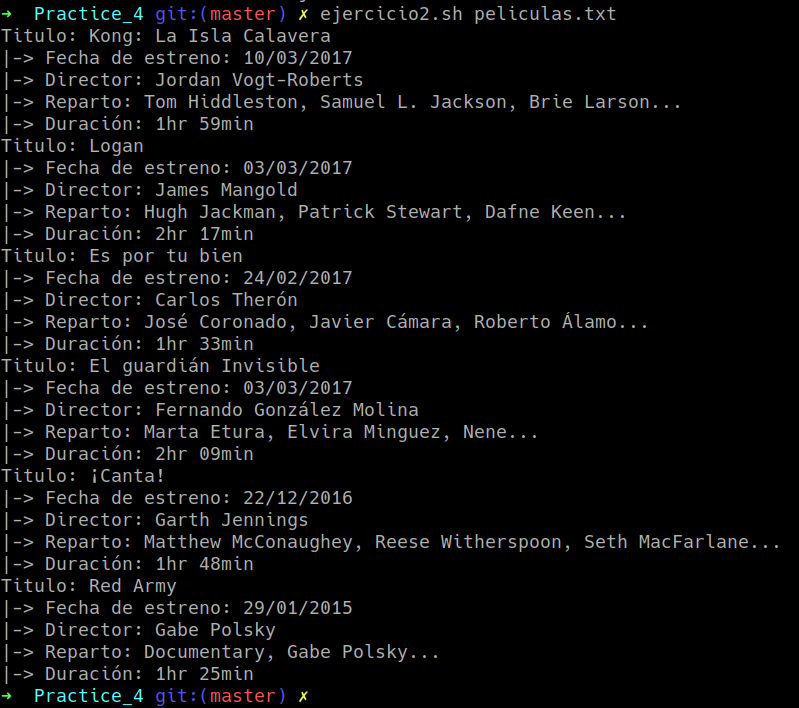
\includegraphics[width=1\textwidth]{images/ejercicio2.png}
\end{figure}

Todos los emparejamientos de las expresiones regulares están explicados en el script a través de comentarios.

\newpage

\section{ejercicio3.sh}
Este script permite un argumento opcional, si recibe más de un argumento se imprime por pantalla un mensaje de error y se abandona la ejecución del script. El primer apartado consiste en aplicar un \emph{grep} que empareje con todos los archivos ocultos de la salida de un \emph{ls -a} en el directorio \emph{home} del usuario que ejecute el script.

La ejecución del segundo apartado varía según si se incluye el argumento opcional. Si se especifica un fichero de texto por línea de comandos. Se hace una copia del mismo eliminando las líneas vacías, haciendo uso de \emph{grep} y el operador \emph{\textgreater}

El tercer apartado utiliza el comando \emph{sed} precedido de \emph{grep} (por razones especificadas en el script) para mostrar algunos campos de los procesos ejecutados por el usuario actual. La expresión regular de este \emph{sed} está detallada en el script a través de comentarios.

\begin{figure}[ht]
	\centering
	\subfloat[Comienzo del apartado 1]{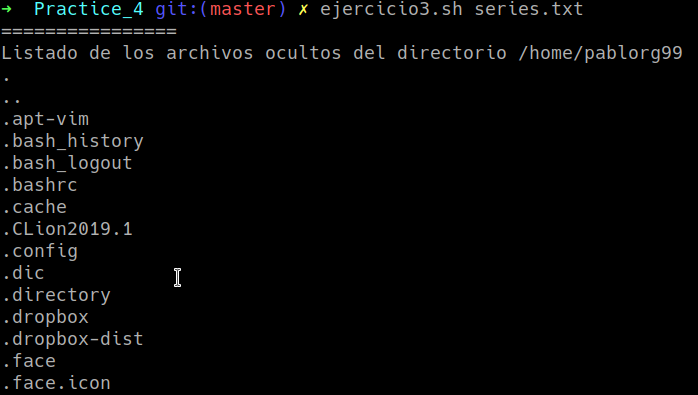
\includegraphics[width=1\textwidth]{images/ejercicio3a.png}}
	\qquad
	\subfloat[Apartado 2 y parte del apartado 3]{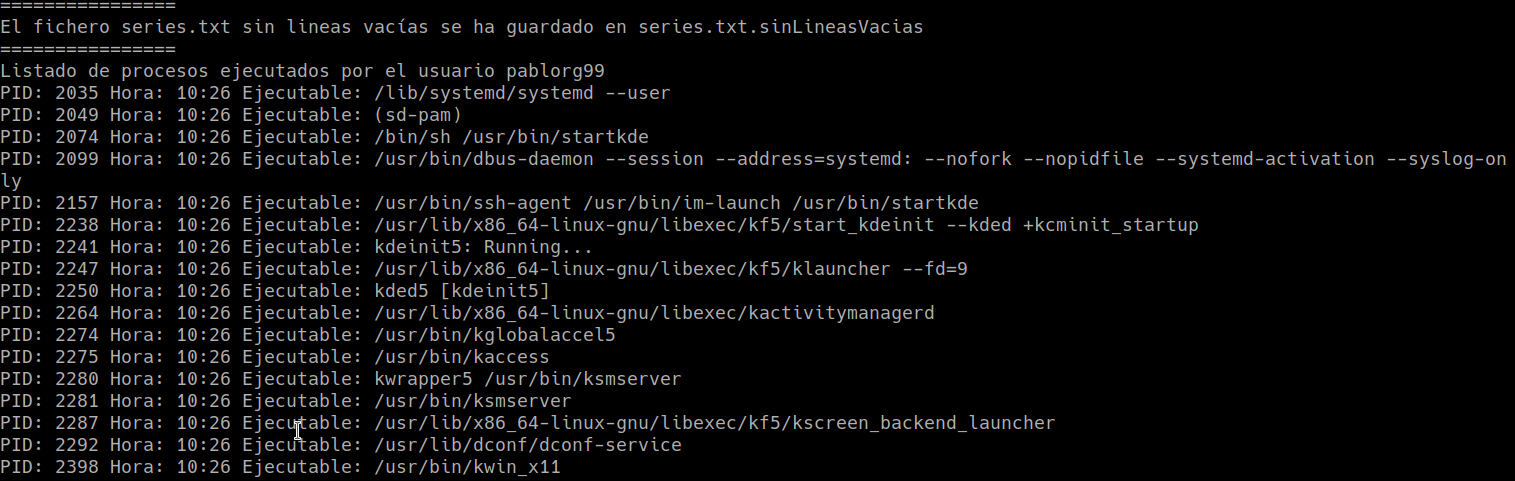
\includegraphics[width=1\textwidth]{images/ejercicio3b.png}}
	\caption{Ejecución del script ejercicio3.sh}
\end{figure}

\newpage

\section{ejercicio4.sh}
Este script requiere dos argumentos, si alguno de estos no se especifican o se introducen de manera incorrecta (el fichero no existe o el número de segundos es un número menor o igual a 0), se termina la ejecución del script. Respecto a estos argumentos, decir que el fichero pasado como argumento será uno que contenga una dirección IP válida en cada línea y que el número de segundos será el que el script usará para determinar que un servidor no ha respondido.

El script hace un bucle en el que en cada iteración, la variable \emph{\$ip} es una línea del fichero pasado como argumento y se utiliza como destino en el comando \emph{ping}. Este se ejecuta con dos opciones: \emph{-c 1} que hace que el ping solo envíe un paquete y \emph{-W}, que como se indica en el propio script, devuelve un error cuando el número de segundos especificado como argumento de esta opción transcurre sin que haya habido respuesta por el servidor. Por último destacar que la sentencia condicional \emph{if} no usa \emph{[ expression ]} porque no evalúa una expresión, sino una variable que se trata como un booleano.

\begin{figure}[ht]
	\centering
	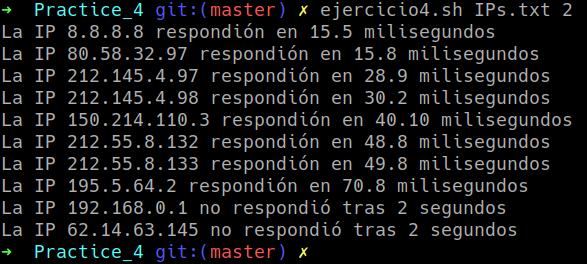
\includegraphics{images/ejercicio4.png}
	\caption{Salida de la ejecución del ejercicio 4}
\end{figure}

El resto de explicaciones concretas del script están documentadas en el código del mismo a través de comentarios.

\newpage

\section{ejercicio5.sh}
El ejercicio 5 no requiere ningún argumento por línea de comandos, se ha añadido una comprobación al inicio del script que avisa al usuario de que este no necesita ningún argumento.

El script consta de tres apartados muy similares. En los tres se hace uso del comando \emph{sed} junto a su comando \emph{s} para formatear el contenido del fichero de cada apartado. Se usan expresiones regulares basadas en el mismo funcionamiento que las del ejercicio 3. El funcionamiento de todo el script está casi unicamente basado en el funcionamiento de estas expresiones regulares, las cuales están perfectamente epxlicadas en el script correspondiente al ejercicio en comentarios.

\begin{figure}[ht]
	\centering
	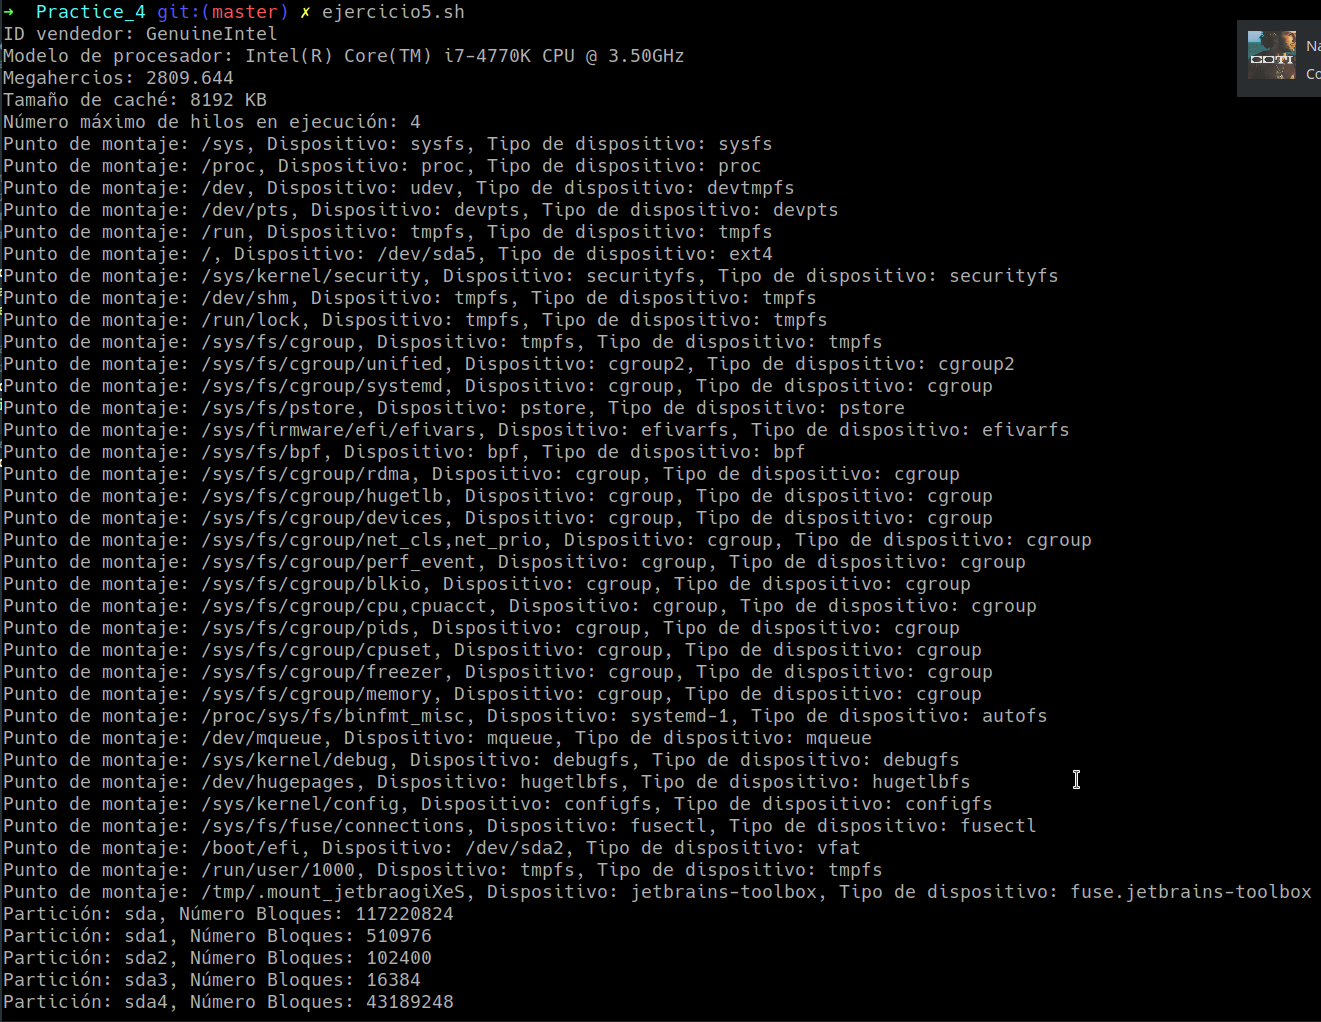
\includegraphics[width=1\textwidth]{images/ejercicio5.png}
	\caption{Ejecución del ejercicio 5}
\end{figure}

\newpage

\section{ejercicio6.sh}
Este ejercicio debe recibir un único argumento, este será la ruta de una \emph{shell}. Si no se recibe un solo argumento se imprime un mensaje de error y se detiene la ejecución.

Se hace uso del comando \emph{grep} para que solo se muestren las líneas que contengan el argumento especificado. Si el script no muestra ninguna información es que no existe ningún usuario con la \emph{shell} especificada. A la salida del grep se le aplica un \emph{sed} con una expresión regular que se corresponde con el formato de la línea. Haciendo uso del comando \emph{s} se establece el nuevo formato.

\begin{figure}[ht]
	\centering
	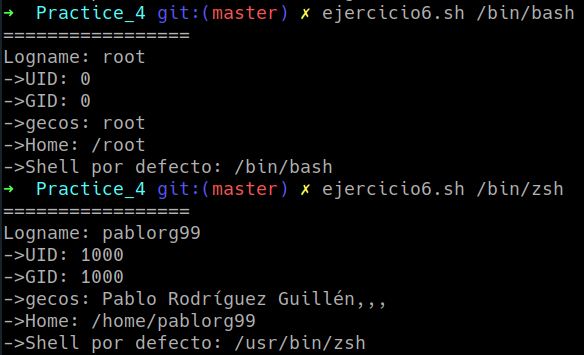
\includegraphics[width=1\textwidth]{images/ejercicio6.png}
	\caption{Ejecuciones de ejercicio6.sh}
\end{figure}


\end{document}
